\documentclass{article}
\usepackage[margin=0.2in,paperwidth=9in,paperheight=4.8in]{geometry}
\pagestyle{empty}
\usepackage{amsmath,amssymb}
\usepackage{tikz}
\usetikzlibrary{shapes.geometric, arrows.meta, positioning, calc}

\begin{document}
\noindent
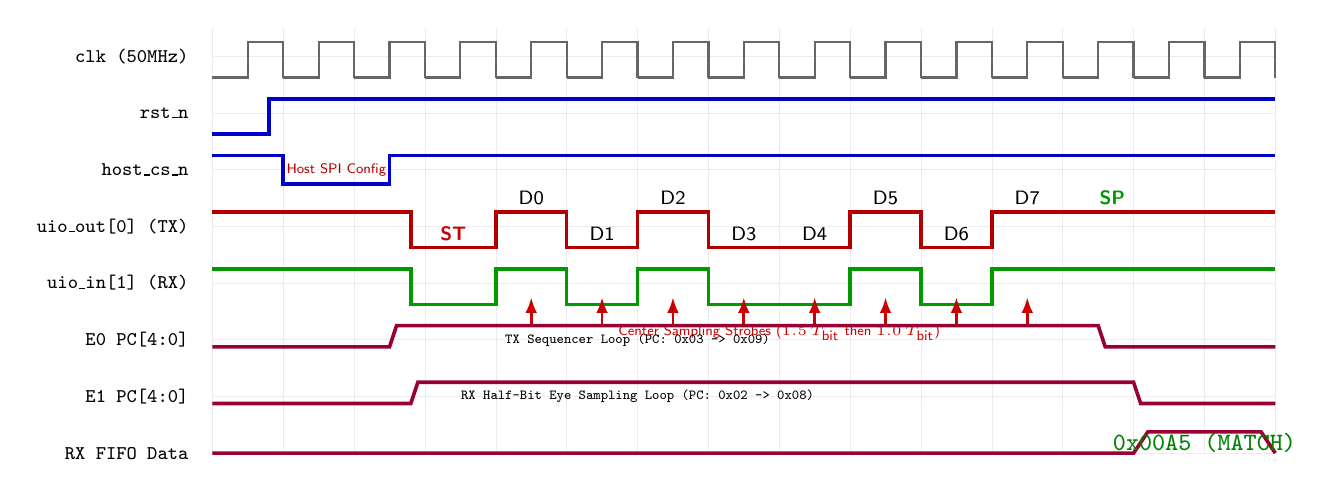
\begin{tikzpicture}[
    scale=0.9,
    clock/.style={line width=0.8pt, black!60},
    sig/.style={line width=1.3pt, blue!80!black},
    tx_sig/.style={line width=1.3pt, red!70!black},
    rx_sig/.style={line width=1.3pt, green!60!black},
    bus/.style={line width=1.3pt, purple!80!black},
    txt/.style={font=\scriptsize\sffamily},
    lbl/.style={font=\scriptsize\ttfamily, anchor=east}
]

% Background grid
\draw[help lines, color=gray!15, ystep=0.8, xstep=1] (0, 0) grid (15, 6.0);

% Labels
\node[lbl] at (-0.2, 5.6) {clk (50MHz)};
\node[lbl] at (-0.2, 4.8) {rst\_n};
\node[lbl] at (-0.2, 4.0) {host\_cs\_n};
\node[lbl] at (-0.2, 3.2) {uio\_out[0] (TX)};
\node[lbl] at (-0.2, 2.4) {uio\_in[1] (RX)};
\node[lbl] at (-0.2, 1.6) {E0 PC[4:0]};
\node[lbl] at (-0.2, 0.8) {E1 PC[4:0]};
\node[lbl] at (-0.2, 0.0) {RX FIFO Data};

% Clock
\foreach \i in {0,...,14} {
    \draw[clock] (\i, 5.3) -- (\i+0.5, 5.3) -- (\i+0.5, 5.8) -- (\i+1.0, 5.8) -- (\i+1.0, 5.3);
}

% rst_n
\draw[sig] (0, 4.5) -- (0.8, 4.5) -- (0.8, 5.0) -- (15, 5.0);

% host_cs_n (pulse configuring baud divisor & pushing 0xA5)
\draw[sig] (0, 4.2) -- (1.0, 4.2) -- (1.0, 3.8) -- (2.5, 3.8) -- (2.5, 4.2) -- (15, 4.2);
\node[txt, font=\tiny\sffamily, red!70!black] at (1.75, 4.0) {Host SPI Config};

% TX line (uio_out[0]): Idle (1) -> Start (0) -> D0(1)..D7(0) -> Stop(1)
% Data = 0xA5 = 10100101 (LSB first: 1, 0, 1, 0, 0, 1, 0, 1)
\draw[tx_sig] (0, 3.4) -- (2.8, 3.4) -- (2.8, 2.9) -- (4.0, 2.9) % Start = 0
             -- (4.0, 3.4) -- (5.0, 3.4) -- (5.0, 2.9) -- (6.0, 2.9) % D0=1, D1=0
             -- (6.0, 3.4) -- (7.0, 3.4) -- (7.0, 2.9) -- (9.0, 2.9) % D2=1, D3=0, D4=0
             -- (9.0, 3.4) -- (10.0, 3.4) -- (10.0, 2.9) -- (11.0, 2.9) % D5=1, D6=0
             -- (11.0, 3.4) -- (12.0, 3.4) % D7=1
             -- (12.0, 3.4) -- (13.5, 3.4) -- (15, 3.4); % Stop=1

% RX line (uio_in[1]): Same as TX (loopback connected)
\draw[rx_sig] (0, 2.6) -- (2.8, 2.6) -- (2.8, 2.1) -- (4.0, 2.1)
             -- (4.0, 2.6) -- (5.0, 2.6) -- (5.0, 2.1) -- (6.0, 2.1)
             -- (6.0, 2.6) -- (7.0, 2.6) -- (7.0, 2.1) -- (9.0, 2.1)
             -- (9.0, 2.6) -- (10.0, 2.6) -- (10.0, 2.1) -- (11.0, 2.1)
             -- (11.0, 2.6) -- (12.0, 2.6) -- (13.5, 2.6) -- (15, 2.6);

% Bit indicators
\node[txt, red!80!black] at (3.4, 3.1) {\textbf{ST}};
\node[txt] at (4.5, 3.6) {D0};
\node[txt] at (5.5, 3.1) {D1};
\node[txt] at (6.5, 3.6) {D2};
\node[txt] at (7.5, 3.1) {D3};
\node[txt] at (8.5, 3.1) {D4};
\node[txt] at (9.5, 3.6) {D5};
\node[txt] at (10.5, 3.1) {D6};
\node[txt] at (11.5, 3.6) {D7};
\node[txt, green!60!black] at (12.7, 3.6) {\textbf{SP}};

% Sample Strobes in RX
\foreach \x in {4.5, 5.5, 6.5, 7.5, 8.5, 9.5, 10.5, 11.5} {
    \draw[-{Latex[length=2mm]}, line width=1pt, red!80!black] (\x, 1.8) -- (\x, 2.2);
}
\node[txt, red!80!black, font=\tiny\sffamily] at (8.0, 1.7) {Center Sampling Strobes ($1.5\,T_{\text{bit}}$ then $1.0\,T_{\text{bit}}$)};

% E0 PC
\draw[bus] (0, 1.5) -- (2.5, 1.5) -- (2.6, 1.8) -- (12.5, 1.8) -- (12.6, 1.5) -- (15, 1.5);
\node[txt, font=\tiny\ttfamily] at (6.0, 1.6) {TX Sequencer Loop (PC: 0x03 -> 0x09)};

% E1 PC
\draw[bus] (0, 0.7) -- (2.8, 0.7) -- (2.9, 1.0) -- (13.0, 1.0) -- (13.1, 0.7) -- (15, 0.7);
\node[txt, font=\tiny\ttfamily] at (6.0, 0.8) {RX Half-Bit Eye Sampling Loop (PC: 0x02 -> 0x08)};

% RX FIFO Data Out
\draw[bus] (0, 0.0) -- (13.0, 0.0) -- (13.2, 0.3) -- (14.8, 0.3) -- (15, 0.0);
\node[txt, font=\small\bfseries\ttfamily, text=green!50!black] at (14.0, 0.15) {0x00A5 (MATCH)};

\end{tikzpicture}
\end{document}
